\RequirePackage{fix-cm}
\documentclass[anonymous,12pt]{iopjournal}
\usepackage{amsmath,amssymb,amsthm,booktabs,array,graphicx,placeins}
\graphicspath{{figures/}}
\hypersetup{hidelinks,pdftitle={Locating dielectric inclusions and choosing a new illumination from finite-aperture scattering data},pdfauthor={}}
\fancyhead[L]{\small\sffamily Inverse Problems\quad Research paper}
\fancyhead[R]{\small Dielectric inclusion tests}
\setlength{\headheight}{17pt}
\setlength{\emergencystretch}{2em}
\renewcommand{\topfraction}{.93}
\renewcommand{\bottomfraction}{.9}
\renewcommand{\textfraction}{.06}
\newtheorem{theorem}{Theorem}[section]
\newcommand{\C}{\mathbb C}
\newcommand{\R}{\mathbb R}
\newcommand{\G}{\mathcal G}
\newcommand{\Bd}{\mathcal B}
\newcommand{\F}{\mathcal F}
\newcommand{\A}{\mathcal A}
\newcommand{\T}{\mathcal T}
\newcommand{\HH}{^{\ast}}
\newcommand{\tr}{\operatorname{tr}}
\newcommand{\diag}{\operatorname{diag}}
\newcommand{\nplus}{n_{+}}
\newcommand{\nminus}{n_{-}}
\numberwithin{equation}{section}
\begin{document}
\noindent{\sffamily\small RESEARCH PAPER}\par\vspace{1.6ex}
\title{Locating dielectric inclusions and choosing a new illumination from finite-aperture scattering data}
\author{}
\begin{abstract}
A limited array can localize a dielectric inclusion without determining the surrounding material. We formulate the output as a set of possible centres and a set of readings that each surviving material class can produce under another illumination. Both are computed from the polarization currents of the nonlinear volume integral equation. Inertia bounds permit invisible current directions and local changes of the material interval admit signed low-rank updates. For two classes, a pair of nonnegative weights bounds the distance between their conditional response sets. Under strict feasibility and a coercivity condition the distance formula is exact for the two quadratic outer sets. A complementary construction gives a lower bound on the incident energy or number of simultaneously controlled transmitters. For specified outlines and contrast intervals in the discrete model, the data exclude 16,313 of 16,384 candidate centres across sixteen 32 by 32 specimens with independently varying exterior contrast. Two further specimens were examined on a 96 by 96 grid. Allowing the edge contrast of the annulus to vary leaves 973 of 9,216 centres possible. Across both grids a two-parameter template fit correctly located all eighteen centres and one fitted material lay inside the data ball. The set method found a compatible full-wave material at all eighteen centres. In two independent native-grid binary examinations, coherent illumination guarantees separation at energies for which every individual direction admits a common reading. At the chosen energy and deterministic error budget two simultaneous directions are necessary and sufficient in one examination. Coarsening the simulation grid changes the field by as much as 5.27 noise radii on the two native specimens. Measured microwave data from two laboratories show how receiver aperture and calibration limit the transfer of a beam chosen from measured fields.
\end{abstract}

\par\smallskip
\keywords{inverse medium scattering, limited aperture, multiple scattering, set inversion, coherent illumination, uncertainty}
\section{Introduction}\label{sec:intro}
A fixed microwave array interrogates a dielectric component. The manufacturing drawing gives a range of possible inclusion sizes and contrasts. The surrounding material is imperfectly known. From noisy complex fields, an inspector wants to know where the inclusion can still be, whether any proposed location has a physically consistent explanation, and whether another exposure would settle a remaining ambiguity. A limit on the error of one fitted image need not answer these questions. They involve all media in a proposed class.

Location and acquisition are linked by the same interior currents. Moving the proposed inclusion changes the local relation between the current and the total electric field. The propagator and the receiving array stay fixed. Changing the transmitted wave changes the current, but the relation between current and field is still imposed by the same dielectric at every illumination. We exploit both facts. A calculation shared across positions supplies an outer cover for the position. For two surviving material hypotheses a second calculation predicts a pair of sets of possible readings. Their distance determines how much incident energy suffices to resolve them under a prescribed error bound. The measured field then updates the surviving classes.

Current-space reconstruction methods separate the component seen by the receivers from a part to be determined by the integral equation \cite{chen,zhong,ffttsom}. Direct and orthogonality sampling methods can estimate a location at low cost \cite{potthast}. Guo and Liu obtain quantitative contrast estimates from multi-frequency backscattering using a Born representation \cite{guoliu}. Our finite-aperture experiment uses a single frequency and retains multiple scattering. Monotonicity methods compare probe domains with far-field operators, in some cases up to a finite number of exceptional modes \cite{griesmaier_harrach,griesmaier_harrach_erratum,albicker}. Our unknown is a spatial class of dielectric coefficients in a specified finite data model. Independent cell values in an inclusion, in a transition layer and in a weakly scattering background form a single hypothesis. Multiple scattering by the background contributes to every reading. We seek a computable outer cover and, where possible, individual full-wave media inside the data ball. This is the exclusion and existence distinction of bounded-error set inversion \cite{sivia}.

Local electromagnetic power laws bound responses in scattering and design \cite{kuang,trivedi,moleskylocal}. Cross-field constraints retain compatibility across incident waves \cite{shim}. We express the material interval as a quadratic form in each current and field row and combine it with the receiver residual. A negative current direction can offset one positive source direction in this relaxation. When the number of exceptional directions is small, the remaining incident fields can still exclude an entire class. In performing many such tests, the quantities to retain are the local current and total-field traces that change when a material hypothesis changes. Related elimination of unchanging variables occurs in static condensation \cite{huynh} and is governed here by Hermitian inertia additivity \cite{haynsworth}.

Illumination for distinguishing two known scattering matrices has a classical solution, the leading incident eigenmode of their squared difference \cite{bouchet}. Selecting inputs that separate set-valued outputs is also familiar from fault diagnosis \cite{scott}. Here the scattering matrix inside a material class is unknown, and old noisy readings constrain the outputs of the same medium on a new illumination. We obtain a two-weight test for the separation of two conditional quadratic response sets. Under stated regularity assumptions the dual gives their exact distance. Exactness concerns these outer sets. Their relation to the physical experiment can be assessed in both directions using full-wave material witnesses and the subsequently measured field.

Sections~\ref{sec:model} and \ref{sec:algorithm} derive the material and acquisition tests and describe their implementation. Section~\ref{sec:exp} examines a limited aperture spanning a $2.67$-wavelength domain, including a weak background that varies independently in every exterior cell. We measure both the size of the location cover and the change produced by a new exposure. A separate two-class experiment compares the energy required by coherent and individual illuminations. Section~\ref{sec:lab} uses scattering data from two laboratories to test how well a beam selected on one receiving arc transfers to another.
\section{A fixed Green operator and two material tests}\label{sec:model}
\subsection{The physical quantities}
Use time dependence $\exp(-{\rm i}\omega t)$ and out-of-plane electric polarization. In a homogeneous nonmagnetic background, the two-dimensional outgoing potential for a polarization current in our normalization has kernel ${\rm i}k^2H_0^{(1)}(k|x-x'|)/4$. The contrast $\chi$ is the excess relative permittivity. Pulse discretization and collocation give the interior Green matrix $G$, the receiver map $S$ and a matrix $\Bd$ of available incident fields \cite{colton,richmond}. For a cell of equal-area disk radius $d$, the self interaction is ${\rm i}\pi kd H_1^{(1)}(kd)/2-1$. The source command matrix $V$ gives $B=\Bd V$. With a real diagonal material $X$ the governing relations are
\begin{equation}
 E=B+GJ,\qquad J=XE,\qquad F_X V=SJ,\qquad
 F_X=S(I-XG)^{-1}X\Bd .                                    \label{eq:tm}
\end{equation}
There are $n$ material cells, $p$ receivers and $s$ measured illuminations. Each column of $J$ is a physical current and each row shares a material value across sources. A material class $\mathcal C$ prescribes $\ell_i\leq \chi_i\leq u_i$, including individual fixed cells. The receiver error has stated bounds in the units of $Y$. For a joint Frobenius radius $r$, a position can be removed if every allowed $X$ has $\|F_X V-Y\|_F>r$. A particular $X$ whose upper residual bound lies within $r$ establishes that the position is possible. Any remaining position must be retained. Statements below about transfer operators assume the forward problem is well posed on the material being considered.

Let $T_i$ extract the two state rows $({\bf e}_i^\top,{\bf e}_i^\top G)$ and let $E_i$ add the incident field to the second row. Thus $z_i=(j_i,e_i)^\top=T_iJ+E_i Z$ with $Z=\binom{V}{Y}$. In this notation $j_i$ and $e_i$ each denote a row over all illuminations. The rank-one material law gives
\begin{align}
 D_i&=\begin{bmatrix}
 w_i &-w_i m_i-{\rm i}\lambda_i/2\\
 -w_i m_i+{\rm i}\lambda_i/2&w_i\ell_i u_i
 \end{bmatrix},
 \qquad m_i=(\ell_i+u_i)/2, \notag\\
 z_i\HH D_i z_i&=w_i(\chi_i-\ell_i)(\chi_i-u_i)e_i\HH e_i\preceq0 .
                                                               \label{eq:cell}
\end{align}
Here $w_i\geq0$ and $\lambda_i$ is real. The latter multiplies the lossless optical equality. The full source matrix in \eqref{eq:cell} retains the interference of the different illuminations at each cell. An unmeasured current can obey one power balance while failing these cross-source conditions.

Add these local forms to the squared receiver residual and write
\begin{equation}
 \A=[S,0,-I]\HH[S,0,-I]+
       \sum_i [T_i,E_i]\HH D_i[T_i,E_i]
   =\begin{bmatrix}K&L\\ L\HH&C\end{bmatrix}.                \label{eq:state}
\end{equation}
On physical currents its compression by $\binom{J}{Z}$ is bounded above by the residual Gram matrix. Define $\A_Z=\diag(I_n,Z)\HH\A\diag(I_n,Z)$ and $\Pi=\diag(0_n,I_s)$. The number of strictly positive or negative eigenvalues is denoted by $\nplus$ or $\nminus$.

\begin{theorem}[Exclusion and reuse of the current states]\label{thm:set}
If $t\geq0$, $jt\geq r^2$, $1\leq j\leq s$ and
\begin{equation}
             \nplus(\A_Z-t\Pi)\geq n+j,                     \label{eq:border}
\end{equation}
the material class misses the noise ball. For nonsingular $K$, let
$Q=C-L\HH K^{-1}L$, $H=Z\HH QZ$ and $\nu=\nminus(K)$. A squared distance lower bound is
\begin{equation}
                 \T_\nu(H)=\sum_{k=\nu+1}^{s}
                      \max\{\lambda_k^\downarrow(H),0\}.       \label{eq:tail}
\end{equation}
For a family changing selected local traces, write
$\A_Z^\theta-t\Pi=A_b+U\HH D U$ at a fixed threshold, and factor
the nonzero part of $D$ as $D=C_D\HH\Sigma C_D$ with $\Sigma$ nonsingular and Hermitian. Both counts are obtained from the fixed augmented matrix construction
\begin{equation}
 \mathcal M=\begin{bmatrix}A_b&(C_DU)\HH\\ C_DU&-\Sigma^{-1}\end{bmatrix}.
 \qquad
 n_\pm(A_b+U\HH D U)=n_\pm(\mathcal M)-n_\pm(-\Sigma^{-1}).
                                                               \label{eq:augment}
\end{equation}
Any verified nonsingular common state pivot can be eliminated first in $\mathcal M$. Its inertia is added back. All other state coordinates stay in the small problem.
\end{theorem}
\begin{proof}
The graph with columns $\binom{J}{I_s}$ has dimension $s$. Its intersection with any positive space in \eqref{eq:border} has dimension at least $j$. Compression to that subspace shows that at least $j$ eigenvalues of the residual Gram are strictly greater than $t$. For nonsingular $K$, completing the square writes the compressed form as $H+P\HH P-N\HH N$ with at most $\nu$ rows in $N$. Interlacing and nonnegativity of the residual Gram give \eqref{eq:tail}. This is sharp for the retained rank information. In the eigenbasis of $H$, choose $N\HH N$ to remove the largest $\min(\nu,\nplus(H))$ positive eigenvalues and take the positive part of what remains. Finally, eliminating $-\Sigma^{-1}$ in \eqref{eq:augment} recovers the updated matrix. Eliminating a common nonsingular state pivot first is another congruence of the same quadratic form \cite{haynsworth,tian,fan}. This argument permits coupled zero modes of the full base or of the update.
\end{proof}

The word ``fixed'' applies to the Green operator and available traces, not to a low-dimensional approximation of every material current. At fixed interval midpoint, narrowing a half-width changes the local quadratic form by a nonnegative multiple of $e_i\HH e_i$. Its update has rank one. A midpoint change can give one positive and one negative auxiliary direction. For a nested interval with a different centre one can also transfer a parent's exclusion by simple set inclusion. A comparison with direct state factorization is meaningful on nonnested intervals whose answer was unknown at the parent.

\subsection{An illumination for two surviving material classes}
For one class let $Q$ be as above. Suppose the matrix of old errors satisfies $D_o\preceq\Omega$. A joint Frobenius bound gives $\Omega=r_o^2 I$. For one old beam this is the scalar $r_o^2$. With several independent column bounds the diagonal of their squared radii does not in general dominate their error Gram. For the old data $Z_o$, put $P_o=Z_o\HH QZ_o-\Omega$. Append a \emph{clean} hypothetical reading $y$ for a command $a$. Its error row and column vanish. The compression proof above implies that
\[
 \nplus\begin{pmatrix}P_o&Z_o\HH Qz\\z\HH QZ_o&z\HH Qz\end{pmatrix}
 \leq\nu,\qquad z=\binom a y .
\]
If $P_o$ is invertible and $\nplus(P_o)=\nu$, the old data already use every available positive exception. The conditional future response satisfies
\begin{equation}
 q(a,y)=z\HH Q_o z\leq0,\qquad
 Q_o=Q-QZ_oP_o^{-1}Z_o\HH Q.                                \label{eq:cond}
\end{equation}
With fewer than $\nu$ positive directions, a single new column can add at most one. The corresponding count alone cannot resolve a larger deficit. Even at saturation the receiving block of $Q_o$ may be indefinite. Counting its bounded directions is not a measure of the separation of two material classes.

For classes $i=1,2$ write $Q_{o,i}=\left[\begin{smallmatrix} A_i&L_i\HH\\ L_i&R_i\end{smallmatrix}\right]$ and let $\mathcal Y_i(a)=\{y:q_i(a,y)\leq0\}$. The distance between these two sets is the smallest difference a clean pair of predicted readings can have in this relaxation. Commands lie in an available subspace with positive power Gram $W$. Its normalization specifies what equal energy means.

\begin{theorem}[Conditional distance and incident energy]\label{thm:power}
For each material class assume that the state $K_i$ and old block $P_{o,i}$ are invertible, $D_o\preceq\Omega$, and $\nplus(P_{o,i})=\nu_i$. With the resulting conditional forms \eqref{eq:cond}, for nonnegative $\alpha_1,\alpha_2$ form
\begin{align}
 D_\alpha&=\begin{bmatrix} I+\alpha_1R_1&-I\\-I&I+\alpha_2R_2\end{bmatrix},
 &B_\alpha&=\binom{\alpha_1 L_1}{\alpha_2 L_2},\notag\\
 H_\alpha&=\alpha_1 A_1+\alpha_2 A_2-B_\alpha\HH D_\alpha^{-1}B_\alpha .
                                                               \label{eq:dual}
\end{align}
Whenever $D_\alpha\succ0$, the squared distance between $\mathcal Y_1(a)$ and $\mathcal Y_2(a)$ is at least $a\HH H_\alpha a$. An incident command with $a\HH H_\alpha a>4r_a^2$ separates the two physical classes for every future receiver error of norm at most $r_a$. At power $E$ the best such bound for fixed $\alpha$ is $E\lambda_{\max}(H_\alpha,W)$ on the allowed subspace.

If both quadratic fibres have strictly feasible points for a fixed command and some choice of weights yields $D_\alpha\succ0$, the supremum of \eqref{eq:dual} is the exact squared distance between these two outer sets. If these conditions hold for all allowed nonzero commands, their optimal one-shot squared separation per unit energy equals $\sup_\alpha\lambda_{\max}(H_\alpha,W)$. For strictly positive finite gain the infimum of sufficient energy for these outer sets is $4r_a^2$ divided by that gain.
\end{theorem}
\begin{proof}
Set $v=\binom{y_1}{y_2}$. Adding $\alpha_i q_i(a,y_i)$ to $\|y_1-y_2\|^2$ and minimizing over $v$ gives \eqref{eq:dual} by completion of squares. The two radius-$r_a$ error balls around any clean pair are disjoint if the squared distance exceeds $4r_a^2$. The energy statement for a trial pair follows by the Rayleigh principle.

For exactness lift $\binom{v}{1}\binom{v}{1}^{\!*}$ to a positive semidefinite complex Hermitian matrix. Its final diagonal entry is one. There are two additional real affine inequalities. Strictly feasible points of the two quadrics yield a strictly feasible lift after a sufficiently small positive perturbation of the top-left block. A positive definite dual state block bounds the trace of the top-left block on every feasible objective sublevel set by completion of squares. The normalized sublevel set is consequently compact. An optimal extreme point of the lifted feasible set exists. If its rank is $h$, a Hermitian perturbation restricted to its range has $h^2$ real degrees of freedom. The at most three active real constraints imply $h^2\leq3$, hence $h=1$ \cite{huang}. Strong duality gives the claimed equality. A dual optimum with singular state can be approached by mixing with a strictly feasible dual point. Finally both optimizations are suprema, and the clean quadratic forms are homogeneous in the pair $(a,y)$. The stated threshold assumes an absolute error radius independent of power.
\end{proof}

There is a converse with physical rather than relaxed content. If actual materials in the two classes fit the old data, with transfer matrices $F_1,F_2$, then for any incident energy $E$ their clean responses differ by at most
\begin{equation}
       \sqrt E\,\|(F_1-F_2)W^{-1/2}\|_2 .                    \label{eq:witness}
\end{equation}
If this is at most $2r_a$ their midpoint is an admissible common new reading for every command at that energy. This limits a worst-case guarantee, while a particular instrument reading may still be decisive. For exact individual transfer matrices the maximizing wave in \eqref{eq:witness} is the known binary discrimination eigenmode \cite{bouchet}. The uncertainty calculation adds a sufficient energy for entire material classes and an experiment capable of testing that prediction. An old-data saturation count alone gives neither endpoint.

\paragraph{One transmitter at a time and coherent hardware.}
A useful lower bound on hardware capability survives adaptive acquisition. Normalize each permitted elementary wave to unit incident power. Suppose the \emph{same} two old-compatible materials admit a common reading $m_j$ on each elementary wave $j$, with errors at most $\kappa_j$. In an adaptive sequence, respond to the selected wave $t_h e_{j_h}$ by $t_h m_{j_h}$. Both materials then produce the same history for the controller. For either one, the squared error of the whole new transcript is at most
\begin{equation}
   \sum_h |t_h|^2\kappa_{j_h}^2
      \leq E\max_j\kappa_j^2,\qquad \sum_h|t_h|^2\leq E.     \label{eq:transcript}
\end{equation}
This proves indistinguishability at a fixed joint absolute error radius whenever $\sqrt E\max_j\kappa_j\leq r_a$. The argument holds for each realization of the controller's random choices. It uses linearity in the illumination of a fixed multiple-scattering medium. Independent stochastic receiver noise that averages down with repeated exposures defines a different experiment.

More generally, for a subset $I$ of simultaneous elementary waves, restrict both $W$ and $H_\alpha$ to their principal submatrices on $I$. A positive lower separation tests sufficiency of that set of transmitters. For the same two physical material witnesses, the largest generalized eigenvalue of $((F_1-F_2)_I\HH(F_1-F_2)_I,W_{II})$ gives a necessary power bound. Taking the largest such gain over the allowed subsets in \eqref{eq:transcript} also covers causal time sharing among sparse coherent commands. The upper and lower tests can therefore bracket the required number of simultaneously controlled transmitters. Enumerating all subsets of size $h$ costs $\binom{m}{h}$ small source problems. The field solve is shared between these problems.

\section{From receiver data to a revised material cover}\label{sec:algorithm}

\begin{figure}[htb]\centering
\setlength{\fboxsep}{5pt}\small
\fbox{\begin{minipage}{.91\linewidth}\centering
Noisy complex responses, a bounded measurement error and a material specification\\
$\downarrow$\\
Apply the common constitutive law across every available illumination\\
$\downarrow$\\
\begin{tabular}{@{}>{\raggedright\arraybackslash}p{.41\linewidth}@{\hspace{.035\linewidth}}>{\raggedright\arraybackslash}p{.43\linewidth}@{}}
\textbf{Position inspection} & \textbf{Two material specifications}\\
Remove impossible centres. Fit a physical material at selected surviving centres and bound its full data residual.
& When both specifications fit the old reading, compare their predicted new fields. Compute necessary and sufficient incident energies.\\[2pt]
Select an additional wave if there is more than one centre. & If the energy permits separation, store the complex weights before transmission.\\
\end{tabular}\\
$\downarrow$\\
Transmit, receive the new complex field, retest the old survivors and report the revised cover or the surviving specification.
\end{minipage}}
\caption{How a new measurement enters the answer. The position inspection uses seven initial waves. The controlled binary experiment starts directly from two specifications and one old wave. Candidate selection can be approximate; removing a material class requires an original-operator lower bound outside the receiver error ball.}\label{fig:workflow}
\end{figure}

\subsection{Searching a field of possible inclusion centres}
Fix a material specification. A candidate centre $c$ translates the prescribed inner core and its boundary layer. Clipping the translated sets at the edge of the field of view includes defects that cross the boundary. For the basic specification a known profile $p_i(c)$ takes values one on the core and one half on the layer. Every occupied cell has its own contrast within $p_i(c)[\ell,u]$. Every exterior cell, including the hole of an annulus, has its own value in $[0,b]$. A second specification allows independent values in $[0,5]$ throughout the boundary layer. A third query allows any one of several named profiles. Its excluded centres are the intersection of the excluded sets for the individual profiles. Centre uncertainty and the area occupied by material are different outputs.

A coarse spatial query can dispose of several centres at once. For a tile of centres $C$ the interval $\ell_i(C)=\min_{c\in C}\ell_i(c)$, $u_i(C)=\max_{c\in C}u_i(c)$ contains the union of their material classes in every cell. If the larger class fails the measurement, remove the whole tile. Otherwise split it, ultimately testing the individual centres with their own narrower intervals. Oversized parent solves can be skipped by passing every descendant to the next level. This property permits early exit from a coarse test without losing coverage. For the fresh comparison we evaluated the remaining leaves directly from the noisy field and included the cost of the parent tests.

For each centre and each material interval, apply Theorem~\ref{thm:set} to the stored complex observation. Retain every outcome for which the distance lower bound is at most the error radius. On retained positions try specific legal full-wave materials and verify their residual with the original Green operator. This gives three possible outcomes for a position: all its materials have been excluded, one compatible material has been found, or its status remains unresolved. For an amplitude query the union of all surviving amplitude bins is an outer bound within the declared material family. Rejecting a translated core does not put a pointwise upper bound on the permittivity at that pixel in every conceivable geometry.

The calculation is practical because the background is common to the whole view. Embed the physical current by zero extension on a doubled Fourier grid and let $\widehat G$ be the stored circulant Green symbol. The same sector inequality holds in the added cells because their physical current is zero and their background interval has lower endpoint zero. Allowing additional currents in the calculation enlarges the relaxation in the safe direction. With unit background weight the material state operator is
\begin{equation}
 K_b=I-b(G+G\HH)/2,\qquad
 \widehat {K_b^{-1}}(\xi)=[1-b\,\operatorname{Re}\widehat G(\xi)]^{-1}.
                                                               \label{eq:pad}
\end{equation}
A positive lower bound on the denominator permits simultaneous calculation of the covariances of current evaluation, interior scattered field evaluation, receivers and incident fields. Translating a local cell pattern reuses the same covariances. Centres that clip differently at the boundary have separate patterns. An interior positive pivot in \eqref{eq:pad} does not force the modified material state or the state after adding receivers to be positive.

For example, with local trace matrix $T$ the update to the state is $T\HH D T$. On a nonsingular active update, the only new material matrix to solve has the form $D^{-1}+TK_b^{-1}T\HH$. Its order is at most twice the number of modified cells. Singular row updates use \eqref{eq:augment}. At each positive scalar residual weight, receiver elimination introduces a matrix of order $p$. The final eigenproblem has order $s$. Its positive spectrum after the inertia penalty gives \eqref{eq:tail}. Adding a further illumination preserves the array and moving cell traces. Only their incident-field and source covariances change. The receive-space implementation and its error control are given in the appendix.

For a truly indefinite common state, precompute its solves against a bank of moving traces and the sources. For $h$ retained nonpivot state coordinates, $q$ active signed trace rows and $s$ sources, each new inertia test then has order $h+q+s$. Dense precomputation with $m$ precomputed trace rows costs order $n^3+n^2m+nm^2$, in addition to storing the Gram blocks. An unrestricted family with $m$ proportional to the whole grid has a substantial offline cost. The localized patterns and the Fourier translation above are two ways to amortize this work. We time both the first search and a repeated search. The small-matrix cost does not include finding the initial material specification.

\subsection{Reinterrogating an ambiguous cover}
The online procedure is described below. A single conclusive outcome is meaningful even if no image is reconstructed. The separate witness search also detects a competing class to which the data really are compatible.

\begin{enumerate}
\item Form the cover from the original noisy measurements. Report verified material witnesses. Stop if the declared task is already resolved.
\item Specify the allowed new source commands and incident power. For a comparison of two classes compute old-conditioned response forms using \eqref{eq:cond}. If there are two old-compatible material witnesses, use \eqref{eq:witness} to test whether the available energy is insufficient to guarantee a decision. Evaluate candidate powers and directions with \eqref{eq:dual}. Record the chosen command, power, noise radius and decision rule before evaluating the unknown material on that command.
\item Take the new reading. For each class minimize its necessary quadratic form over the measurement's receiver noise ball. A strictly positive lower bound excludes that class. Try specific material witnesses against both readings. For a spatial cover, apply the joint old and new current test at every remaining centre. Keep every old exclusion.
\end{enumerate}

For many retained centres, computing pairwise conditional forms at every location can dominate the search. We examine a cheaper design rule in the location experiment. Select up to twenty representative centres using evenly spaced ranks in raster order. Compute the full-wave transfer at the nominal core contrast and a legal vacuum background for each. Among individual angles and the coherent eigenmodes of each representative pair, choose the command that maximizes the smallest nominal separation across those pairs. Representatives affect source proposals only. Every centre in the original cover is tested after the new measurement. The comparison includes the best single angle chosen by the same score. This matters when the array already has an individual transmitter near an effective coherent mode.

For two material classes the search for multipliers uses actual old readings and a public model for each allowed box. In distorted-current coordinates $h=J-ME$, where $M$ is the diagonal midpoint material, the exact future field is affine in $h$. The necessary sector reads $\|h a\|^2\leq\|W_h E a\|^2$ for every source vector, where $W_h$ contains the spatial half-widths. Concentrating an additional signed optical weight on a cell changes the state by at most two rows. We screen state weights with the clean projected separation in the direction joining the two nominal responses. Two nonnegative weights then optimize \eqref{eq:dual} in the source subspace, using the actual incident-power Gram. The resulting eigenvector and dual weights are proposals. Strict separation requires an independent, one-sided evaluation on the original operator. A positive-state fit, single-beam choices and the known-pair coherent optimum use the same powers and receiver error. This comparison measures which part of any gain comes from coherent illumination and which part comes from controlling material uncertainty.

\section{Location and illumination at full wave scale}\label{sec:exp}
\subsection{The inspection question and the comparison}
We use a two-metre square in air at 400 MHz. Its side is 2.67 free-space wavelengths. A pixel in the 32 and the 96 discretizations has side 62.5 and 20.8 mm, respectively. A separate seven-wave inspection of each spatial target spans 135 degrees of incidence. Nine observation angles span 146.25 degrees. There is no access to the opposite arc. The task is to locate a dielectric part from a set of possible outlines, within known tolerances on contrast and in an imperfectly known background. Outside the indicated material the background can vary independently in every pixel, from zero to $b=1/32$. The interior of a hole has this same uncertainty. A companion measurement uses the same inclusion with vacuum outside. We compute the field with the full nonlinear operator throughout. At 32 points per side the norm of the difference between the Born and full-wave data, divided by the full-wave norm, ranges from 176 to 361 percent. For the two native targets the range is 214--304 percent.

Sixteen independently generated specimens at the first resolution comprise four each of a disk, an annulus, a pair of inclusions, and an annulus with satellites. The poses and internal texture vary within each family. Two additional native-grid specimens have a ring centred at pixel $(29,66)$ and a pair centred at $(94,33)$, indexed from zero. The second pair extends past the right boundary. All positions, including edge-clipped positions, are tested. A position denotes the anchor of the specified shape, so excluding it makes no assertion that the material at that single pixel is vacuum. We use the entire noisy complex matrix and a common Frobenius error radius. A point in a retained cell of the map can have either an explicitly realized material or an unresolved existence test.

The beams used to examine two alternative amplitude patterns form a separate population. The two alternatives share a strong dielectric body and differ on two weakly uncertain lobes. They have the same permitted active region. There are 16 incident elementary waves and 16 receivers on a 168.75-degree aperture. The first illumination is available to every design, leaving 15 directions. The candidate-centre transfer contrast determines a useful empirical control; only the full intervals and old measurements enter the bounds on all materials. We distinguish a development group, enriched for a future gap near the noise, from a confirmation group selected using old data alone. The latter contains 12 independent 32-grid specimens and two independent 96-grid specimens. All policies on a specimen receive the same energy and the same absolute receiver error allowance. Apertures, noise draws, transmitted beams, and repeat exposures are paired conditions on these objects.

\subsection{What the old measurements locate}
Table~\ref{tab:cover} gives whole-field results for a specified shape. A verified material was found at every generating centre in the primary tests. For the sixteen 32-grid specimens, the largest cover contained twelve cells and the smallest one. Using all four possible outlines together, all 48 alternatives with incorrect shape were excluded at every centre. For the correct outline, the centre cover and its witness were unchanged. Scanning a single full-wave material template at the midpoint of the specified inclusion interval with vacuum outside ranked the generating centre first on all sixteen smaller specimens and on the native annulus. On the clipped native pair it ranked the generating centre second, one cell away from its preferred position. Even the best nominal point residuals were 3.61--6.81 noise radii on the smaller grid and 4.54--5.29 on the native grid. We therefore fitted a common core amplitude and homogeneous background on the five best nominal centres of every specimen. The selected positions recovered all eighteen centres, including the clipped pair. The fitted residuals at the two native centres were $1.0043r$ and $1.0094r$ (in ascending order); only one of eighteen fitted media passed full-wave error verification. This fit used 3,151 full-wave point evaluations, with 68.69 seconds for fitting and 0.52 seconds for independent readback on the same machine, in addition to the original template sweep. Allowing spatially varying material then yielded a witness at all eighteen centres. These comparisons give no point-location advantage to the set method. They distinguish a correct centre from a physically admissible dielectric and from a bound on all alternative locations. An orthogonality-sampling backpropagation indicator placed its largest value at the generating centre on three specimens and placed it within its five highest pixels on five. This indicator ranks pixels by a physical correlation. Without an independent outer error bound on the rank it provides a different output from a set containing all possible centres.

\begin{table}[tb]\centering
\caption{Possible inclusion centres before a further exposure at 3 percent noise. The discrete model and the stated outline and contrast intervals are assumed here. An exclusion applies to every material in that class. The witness column counts centres with a checked material. Unresolved centres are retained. Alternative specifications on the same specimens are paired conditions.}\label{tab:cover}
\small\begin{tabular}{@{}lrrrr@{}}\toprule
Material class and grid & Tested & Excluded & Witness & Unresolved\\\midrule
Specified layer, sixteen $32^2$ & 16384 & 16313 & 16 & 55\\
Specified layer, $96^2$ annulus & 9216 & 9099 & 1 & 116\\
Specified layer, $96^2$ clipped pair & 9216 & 9192 & 1 & 23\\
Uncertain layer, four $32^2$ annuli & 4096 & 2381 & 4 & 1711\\
Uncertain layer, $96^2$ annulus & 9216 & 8243 & 1 & 972\\\bottomrule
\end{tabular}\end{table}

To isolate the effect of an uncertain background we evaluated the receiver-direction perturbation bound at the same centres. With the exterior known to be vacuum it excluded 16,301 of 16,384 centres, compared with 16,349 using the combined tests. Allowing each exterior cell up to $1/32$ left the perturbation test without a single exclusion. The inverse of the centre-field propagator still exists, but the absolute majorant for scattering by the exterior is too large. The material sector treats exterior power jointly before taking a receiver norm. This difference is substantial even for a weak background; it does not establish failure of every possible perturbation inequality.

Widening the material tolerance reveals the role of the negative current space. The primary inspection specifies a half-amplitude boundary layer around each core. In the wider inspection the core cells vary independently in $[3,5]$ and the boundary cells independently in $[0,5]$. The four 32-grid annuli then give 555, 568, 616 and 642 excluded centres. The successful state matrices have two to five negative directions. On the native annulus, all 8,243 strict exclusions in this wider class use an indefinite state. Relaxing the boundary description makes the potential positions more numerous even with unchanged readings.

A zero count from a finite positive-weight search need not indicate a physical obstruction. We therefore compare with continuously variable nonnegative weights on the background and the footprint. At one tested annular position the continuous search found a positive state whose verified distance lower bound exceeded the receiver radius by $0.5927$. At one different position of each of the four 32-grid annuli we exhibited a nonzero current in the exact receiver null space. Both its footprint-sector and background-sector energies were strictly negative on the original operator. Any nonzero nonnegative combination has a negative direction at that position, for every positive overall scale and every positive semidefinite receiver weight. The indefinite test excludes all four positions. This identifies both an actual obstruction and an example where a better positive search succeeds. Independently varying optical weights at every pixel constitute a larger comparison class.

\begin{figure}[tb]\centering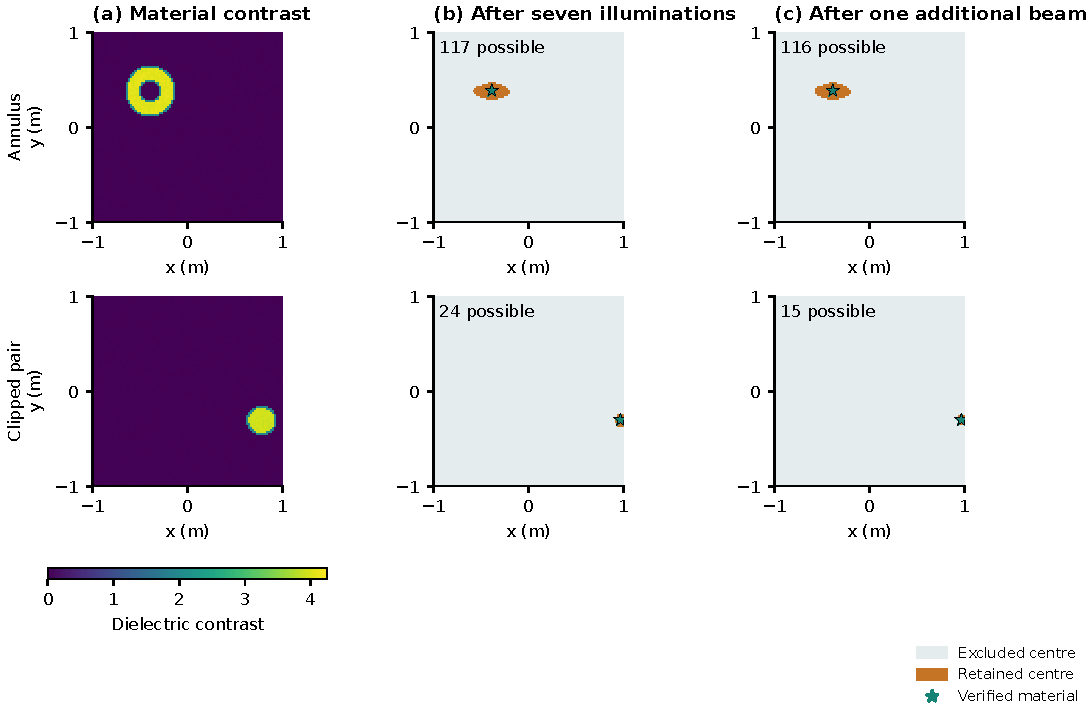
\includegraphics[width=\linewidth]{location}
\caption{Whole-field tests on the two 96 by 96 specimens. The first column gives the generating material for scoring. The central column uses seven old illuminations. Orange cells retain a possible centre and the star denotes a centre with a verified material. The final column uses one further coherent illumination. In the clipped pair the admissible region lies against the outer boundary. All three panels in a row have the same spatial extent.}\label{fig:loc}
\end{figure}
\begin{figure}[tb]\centering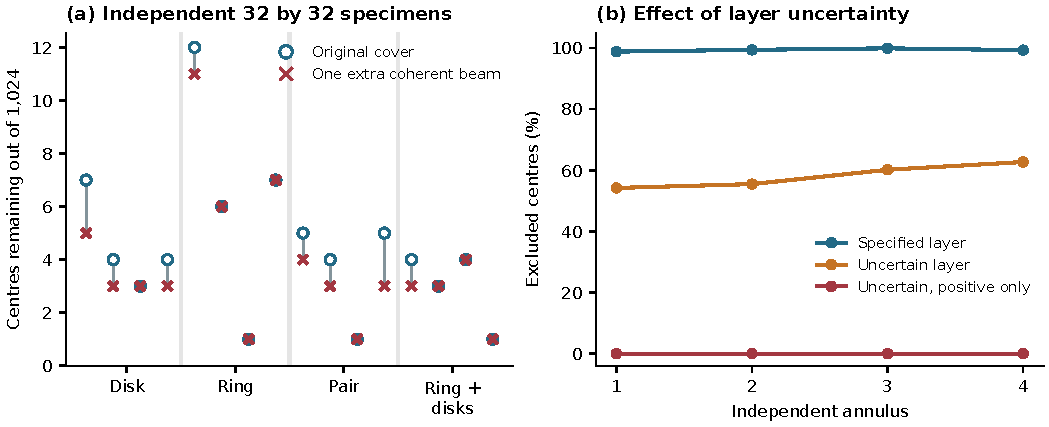
\includegraphics[width=\linewidth]{population}
\caption{Location cover and material tolerances. Left, each pair of marks belongs to one independent specimen with uncertain exterior. Right, the reduction in excluded centres when boundary contrast is released. The positive-state curve uses the same finite menu restricted to positive states. The continuous-weight comparison in the text addresses the limitation of this control.}\label{fig:population}
\end{figure}

A position test also permits a conditional amplitude question. We retain the shape and pose and replace the amplitude specification by adjacent intervals. At the native annulus the interval $[2,3]$ and the interval $[3,3.75]$ for the core profile are inconsistent, while a material in $[3.75,4.25]$ fits the data. A box constraining every core value to the same interval asks a different question from bounding an arbitrary isolated pixel. For example, failure of the low box means at least one value exceeds its upper endpoint, conditional on the other geometric and material constraints. A separate independent-cell peak-cap test at the returned centre gives a strict lower bound of 3.0 for the native annulus and 2.5 for the clipped pair. The upper bound remains at the imposed maximum of 6.0. Each has a witness with peak 4.25. The detector cannot assign the largest value to an individual pixel. A more permissive task must also test mixtures that straddle the bin boundaries.

The noise sensitivity in Figure~\ref{fig:phase} uses one predetermined specimen of each 32-grid shape and both native specimens. New complex noise draws share the physical targets. On the first grid we re-evaluate all the centres. On the native grid we transfer the strict 3 percent distance lower bound $d_3$ using the 1-Lipschitz dependence of a distance on the observed field: $d(y')\geq d_3-\|y'-y_3\|_F$. This conservative alternative avoids recomputing clipped edge geometries. At 10 percent in the unknown background the two native counts are 8,903 and 9,177 strict exclusions. At 1 percent the original native witnesses failed the tighter transfer check. Refitting them on the noisy readings gave verified residuals below 0.863 and 0.753 of the new radius for the two weak-background specimens. Physical witnesses were found on both grids for all 36 paired background and noise conditions. The noise figure counts physical centres across paired targets, including any unresolved cells.
\begin{figure}[tb]\centering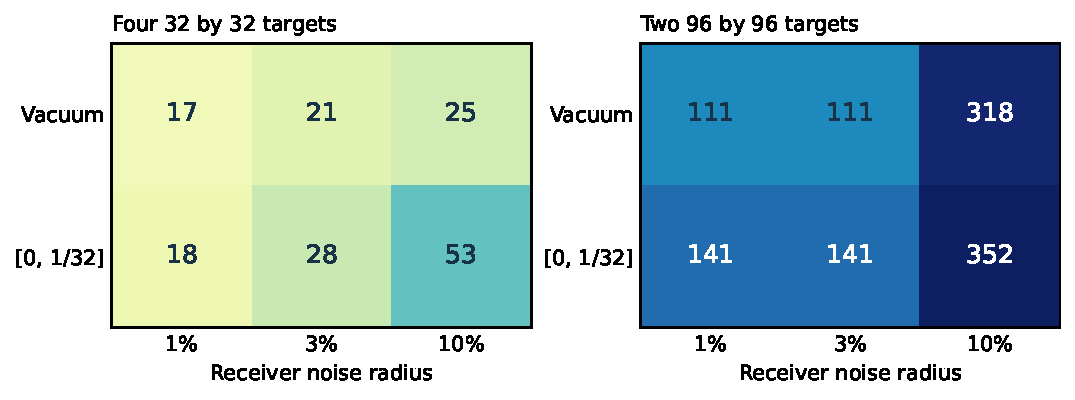
\includegraphics[width=.93\linewidth]{noise_phase}
\caption{Numbers of centres retained over the whole field as background uncertainty and receiver noise change. Each row represents data generated in the indicated background, and inversion uses the matching background contract. The denominators are 4,096 on the left and 18,432 on the right. Full recomputation on the left and a transferred native bound on the right have different sensitivity to lowering the noise.}\label{fig:phase}
\end{figure}

\paragraph{How much a change of discretization costs.}
To test the effect of resolution, we also average each of the two native materials over $3$ by $3$ blocks and solve a new 32-grid volume integral equation with the same physical sources and receivers. Coincident incident fields agree to $9\times10^{-16}$ relatively. Receiver rows are expressed in the native angular quadrature units. Relative to the clean 96-grid measurements the differences are 15.82 percent for the annulus and 6.77 percent for the clipped pair. They amount to 5.27 and 2.26 times the stipulated receiver error. Against the actual noisy readings the coarse solutions give residuals of 5.28 and 2.44 noise radii. Adding these sample discrepancies to the original radius would require factors 6.28 and 3.26 after rounding upwards. These are measured discrepancies for two materials. A model-error bound covering the whole material class would be required to transfer an exclusion between grids.

\subsection{Costs of an indefinite position or amplitude update}
To measure the cost of changing a box we use two arrays for which the common parent gives an unresolved answer. One has 1,024 state coordinates and seven negative directions. The second has 9,216 electromagnetic cells and 1,153 possible current cells with nine negative directions; the remaining cells are exactly vacuum in this timing experiment. Width and midpoint changes at three locations give a rank-four signed update. There are 1,000 distinct, nonnested changes on each specimen, of which 757 and 472 are excluded, respectively. Counts from the reduced matrices agree with direct original-state computations for all the changes. Four predetermined changes on each grid undergo a separate original-operator interval evaluation. An exactly singular control with a null current coupled to a source exercises the retained border in \eqref{eq:augment}.

Two full-wave amplitude controls put the widths in context. A low-contrast disk (peak $0.625$) and a hollow ring (peak $3.50$, first-Born field error $376\%$) occupy the same permitted 1,153-cell circular region, with different actual supports. Against the same solid tapered specification centred at peak four, the excluded widths are approximately $5.14$ and $3.09$ times the Neumann norm cutoff, respectively. In each case a permitted perturbation has spectral radius above one (lower bounds $1.086$ and $1.389$). These fixed-position controls are separate from the whole-field location cohort.

For the first grid the first hundred original factorizations took 52.4 seconds and the thousand took 870.6 seconds. Once the common matrices were prepared the corresponding 128-bit reduced runs took 0.090 and 0.955 seconds. Including common input, setup and all thousand reduced checks costs 96.7 seconds. Adding the four independent original-state interval checks increases the cost to 382 seconds. The measured original-state and reduced floating-point CPU times for the thousand changes are 582.9 and 0.117 seconds. For the second grid a thousand direct numerical factorizations took 1,157 seconds and the prepared interval updates took 5.56 seconds. With all preprocessing and four original-operator checks included the cost was 342 seconds. At just a hundred tests the fully charged reduced runs were slower on both grids: 234 versus 52 seconds and 238 versus 83 seconds, respectively. The amortization becomes visible only after enough changes have been tested. These paired timings concern equal inertia decisions at the same threshold. They do not compare the time to a reconstructed image. On both grids an admissible upper-endpoint perturbation had spectral radius strictly above one, with respective lower endpoints 1.0010 and 1.1083. A centre-series contraction in any induced norm therefore fails for that perturbation.

A fresh multiscale comparison used four predetermined 32-grid specimens and both native spatial specimens with uncertain background. A strict parent test removed 1,740 of 4,096 centres before individual testing on the first grid and 9,359 of 18,432 on the second. All 3,361 successful parent tests had a negative state direction. For the native annulus alone, 366 groups of nine centres were excluded in one test per group. Evaluating the remaining leaves anew gave exactly the same complete cover as an independent scan of every leaf, on every specimen. All six full-wave witnesses survived. The individual centre--weight evaluations fell from 4,208 to 2,468 and from 18,714 to 9,355, respectively. With identical shared state preparation, the measured online times for grouped versus flat evaluation were 8.45 versus 3.71 seconds over the four smaller targets and 78.92 versus 29.04 seconds over the two native targets. Within the native multiscale run, 51.07 seconds were spent factoring the parent classes. With the common state and clipping preparation charged, the totals were 247.57 versus 197.69 seconds. Forming the wider spatial classes costs more than the saved leaf tests on these arrays. For this application we use direct translated tests when online latency is the objective.

A whole-field position scan has a different setup cost. The native annulus has 625 distinct clipped edge geometries. Computing location-independent state information for the primary native annulus took 317 seconds; the subsequent port calculations for the two background measurements took 62 seconds together. Reusing an interior plan for the wider annulus required 103 seconds for the original interior calculation and a further 282 seconds for the full field. Charging both prevents the inexpensive repeats of one fixed local change from standing in for the cost of a new geometry.

\subsection{The value of a further illuminated field}
For location alone the three already unique 32-grid covers need no further exposure. On the other thirteen, an additional uniform direction left all 68 old possible centres. A random angle left 66, the best individually selectable angle left 57 and coherent illumination left 58. The last two designs used nominal responses of representatives in the old cover; every previously retained centre was tested after the acquisition. All four policies retained every generating centre. For all sixty follow-up observations a full-wave material at the returned centre fits the two separate error balls. The original material sufficed in 49 measurements; a bounded refit at the same centre sufficed in the remaining eleven. The maximum verified residuals were 0.988 and 0.979 of the old and new radii, respectively. The native clipped pair changed from 24 possible centres to 18 under uniform incidence and to 15 for either optimized choice. For the annulus its 117 possible centres changed to 116 under uniform incidence, 115 with the best single angle and 116 with the coherent wave. A favourable beam for discrimination of two classes need not be favourable for many adjacent positions.

We next ask a question for which a guaranteed improvement in the reading has operational significance. Can a single acquisition distinguish two surviving material specifications for \emph{all} admissible new errors? At a preliminary common fluence of $0.014$ old-shot units, a verified physical pair in each of the fourteen confirmation cases had full-dictionary maximum difference below $2r_a$. Changing the beam alone could not meet that demand. We then used only the old data and a stored pair of indefinite conditional forms to set the energy for a target separation of $2.15r_a$. The energy is common to all competing policies within each specimen. The twelve energies at the first resolution ranged from 0.0352 to 0.491, with median 0.0778. The two native energies were 0.1778 and 0.4200. All cases had one negative state direction and one positive old-data direction per material class. The old-data-conditioned bound exceeded $2r_a$ in all fourteen, and a new measured field eliminated the wrong class in all fourteen. Forward evaluation gave a material in the surviving class each time. These counts at target-selected energies should be read together with the independent necessary-energy bounds in Figure~\ref{fig:energy}.

\begin{figure}[tb]\centering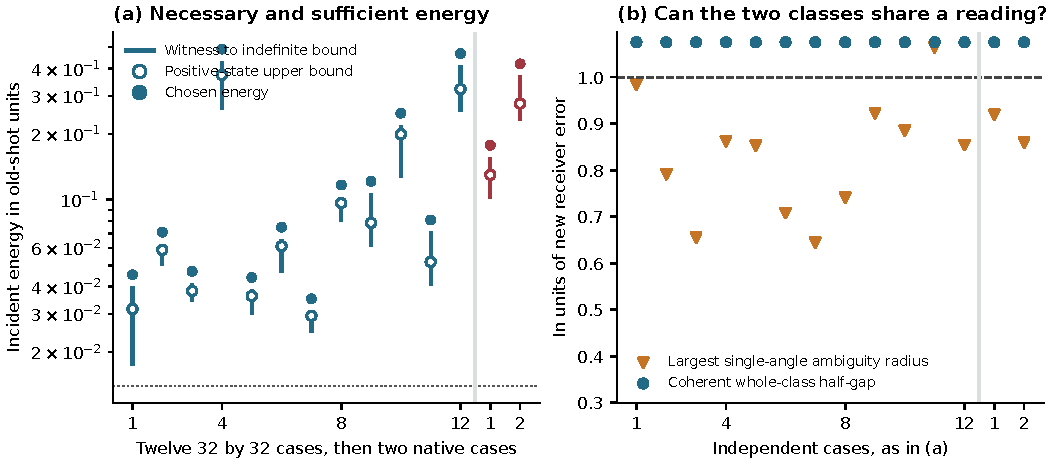
\includegraphics[width=\linewidth]{energy}
\caption{Paired incident-energy comparisons on the fourteen confirmation specimens. Left, lower endpoints use actual old-compatible materials; upper endpoints use whole classes and the indicated state. Filled dots give the energy used before recording a new field. Right, an orange value below one establishes a common reading for \emph{every} elementary angle, while a blue value above one guarantees separation under the coherent command. The vertical divider separates the grids.}\label{fig:energy}
\end{figure}

The necessary and sufficient energy brackets obtained with the indefinite forms are $[0.1034,0.1539]$ and $[0.2344,0.3636]$ for the two native specimens (endpoints rounded outwards). The lower endpoint uses two physical materials compatible with the same old reading. The positive-state calculation improves the sufficient endpoints to 0.1302 and 0.2761, rounded upwards. The classical coherent wave from the two centre transfer matrices, evaluated with the same positive form, already gives sufficient energies of 0.1335 and 0.2831. The numerical evidence supports a benefit from coherent hardware and from reasoning about material classes. It does not establish an advantage in reconstructing material over the classical eigenwave of two known transfer matrices.

With a single transmitter at a time, common readings exist on all fifteen admissible directions in eleven of the twelve 32-grid cases and in both native cases, at the very energy used by the successful coherent command. On the remaining small-grid specimen the result covered thirteen of fifteen directions. For the native specimens the largest upper bounds on the common-reading error over all angles were 0.9191 and 0.8590 times $r_a$. Equation~\eqref{eq:transcript} extends this obstruction to time sharing at fixed total incident energy and one joint receiver error budget. It is independent of which measured field happened to be drawn.

On the actual measurements, in contrast, the best Fisher angle and the centre-discrimination eigenwave both selected the correct class on all twelve 32-grid specimens and both native specimens when either of the same two verified forms could exclude a class. With the indefinite form alone the Fisher, uniform and random counts on the first grid were seven, eight and two. Uniform and random directions each succeeded on eleven of twelve and on both native specimens. This observation is consistent with the common-reading counterexamples: set separation protects against an adverse reading, whereas a particular noise draw can be easy to classify. Additional diagnostic calculations in the development group were used to adjust state weights. Their success rates are not pooled with confirmation.

Finally we asked how many elementary waves must be driven \emph{simultaneously}. On the first native specimen one transmitter is insufficient and three suffice, giving a minimum of two or three. On the second specimen the exact minimum is two. A command on the directions $67.5$ and $90$ degrees has a strictly positive gap of $0.0921r_a$ after subtracting both error radii. A receiver-direction projection of the full-wave real material secant, including its bounded higher-order remainder, sharpens the quadratic test on this borderline pair. Independent native-operator norm enclosures for the two classes of the second specimen give $\eta<0.01438$ in \eqref{eq:realwidth}. The two native three-transmitter quadratic distances are at least $2.1026r_a$ and $2.1095r_a$. In one 32-grid case all 455 triples admit a common physical reading and a four-transmitter distribution gives $2.0200r_a$, proving a minimum of four. Thus the hardware question can have a definite answer even while much of the material remains undetermined.


\begin{table}[tb]\centering
\caption{Three sparse-hardware results at the chosen incident energy. The impossibility column uses an old-compatible physical pair for every indicated subset of transmitters. The two remaining columns concern the entire material intervals. A successful realized readout alone contributes nothing to the necessary count.}\label{tab:ports}
\small\begin{tabular}{@{}llll@{}}\toprule
Specimen & Insufficient simultaneous ports & Sufficient & Minimum\\\midrule
$32^2$, case three & every triple (455/455) & 4 & 4\\
$96^2$, first & every individual (15/15) & 3 & 2--3\\
$96^2$, second & every individual (15/15) & 2 & 2\\\bottomrule
\end{tabular}
\end{table}

The full-wave witness upper bounds on two-port capability were also evaluated on all 105 pairs on each native specimen. They ruled out 100 pairs for the first and 97 for the second. With the second specimen the real-contrast receiver projection in \eqref{eq:realwidth} proved four of the eight remaining pairs sufficient. After committing these restricted commands, new full-wave readings retained a physically realized true class on both specimens and removed the false class even on the first specimen, for which two-port sufficiency is still unresolved. Computing all candidate support scores of sizes one through four and the full set, from cached quadratic forms, took 1.06 seconds for the two native cases. The physical witness bounds took a separate 4.75 seconds, and refining the two-port real-contrast receiver directions took another 4.76 seconds. Original-operator evaluation of the fourteen experiments, including competing policies and their readouts was considerably more expensive: the twelve small-grid objects took 38.3 seconds and the two native objects 132.3 seconds. These costs include the numerical verification and are separate from measurement energy.

\section{Laboratory measurements and model discrepancy}\label{sec:lab}
An additional computational test uses the complex microwave measurements of the Institut Fresnel and the University of Manitoba \cite{fresnel,manitoba}. The underlying physical specimens consist of three dielectric configurations with foam and dielectric inserts at Fresnel and four dielectric objects at Manitoba. They are useful for two questions that a matched discrete simulation cannot address: how an illumination transfers to receivers outside the design arc, and how much modelling error an exclusion claim can tolerate.

For each laboratory and frequency take every unordered pair of its specimens. Use the measured response difference on one half of the common receiving aperture to select a unit-norm coherent combination of the available incident columns. Select the strongest individual column on that same half as the control. Compare their measured complex-field differences on the opposite half and exchange the halves. Fresnel has two common source directions, at $0$ and $180$ degrees. At Manitoba twelve transmitters alternate with twelve receivers around the array. Source normalization is Euclidean in the recorded coordinates. At each frequency the two halves, and the pairs that share a target, are correlated conditions. This retrospective use of the measured matrices estimates transfer across receivers. A calibrated input power Gram and an independent physical replay would be needed to convert it into a transmit-energy experiment.

At Fresnel the coherent combination gave a larger held-out difference in 17 of 18 conditions at 4, 6 and 8 GHz. With the individual empty reference the median ratio was 1.088 and the range was 0.995--1.266. Replacing those references by a common empty reference gave 1.088 and 0.993--1.266. At Manitoba, using the larger metal reference and the initial empty acquisition, the corresponding count was 45 of 84, the median was 1.021 and the range was 0.350--2.741. Calibrating with the smaller reference reduced the count to 32 of 84, with median 0.877. Figure~\ref{fig:lab} shows the full distribution. A commanding improvement on the design half can disappear on the held receivers. Calibration choice is especially important for the second apparatus.

For a nonlinear material bound the error ball must include the loaded instrument and discretization discrepancy. In a previously evaluated contrast test, the large nylon cylinder at 3 GHz left a margin of $4.018\%$ of the observed norm after reference errors were allowed for. Only a loaded discrepancy below that margin would permit exclusion of all media with contrast at most one. Fitting the empty chamber does not supply such a uniform bound. The nonnegative Born residual exceeded the empty-field reference error in 3 of 9 Fresnel and 25 of 28 Manitoba object--frequency conditions. These finite comparisons describe the scale of model error. They do not establish a measured inclusion-location or classification guarantee.
\begin{figure}[tp]\centering
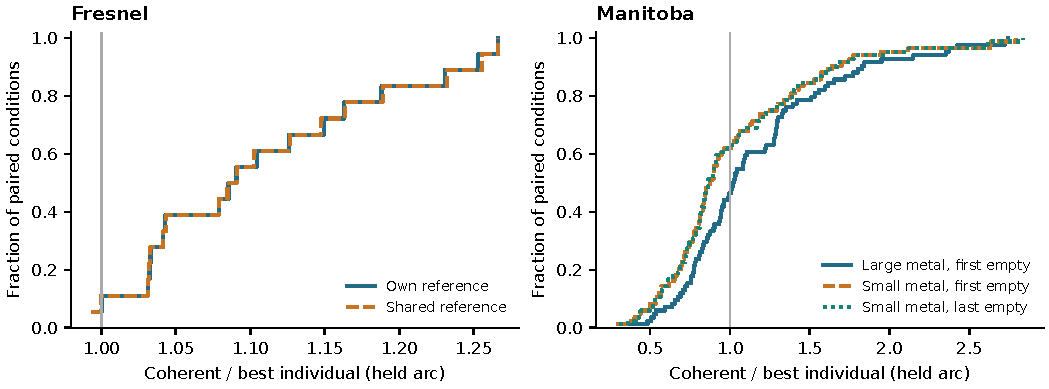
\includegraphics[width=.94\linewidth]{measured}
\caption{Held-receiver field differences for two measured specimens, normalized by the field difference of the strongest individual transmitter chosen on the design arc. The central line denotes equal performance. Each distribution counts pair, frequency and receiving-split combinations. Recalibration of the Manitoba data changes the ranking while leaving the physical specimens fixed.}\label{fig:lab}
\end{figure}

\section{Discussion and conclusion}\label{sec:discussion}
For the specified inspection task the outputs are a spatial cover, individual physically admissible examples, and a decision about another measurement. The two theorems use the same material law in different ways. Across positions the invariant object is the fixed propagation operator and the changing quantities are a few local constitutive traces. Across illuminations the invariant object is the unknown common material and the changing quantity is the applied field. Receiver-null currents account for both the failure of a positive-state test at certain positions and the limited information available from a single direction.

Three distinctions affect how these results can be used. First, a smaller position cover can be purchased with a tighter drawing or with a new measurement. Reporting the two effects separately reveals how much the measurement actually contributes. In particular, the dramatic full-field reductions in the original seven-wave experiment coexist with modest improvements after an eighth wave. Second, illumination power must be specified on the admissible source dictionary. One port used for longer and two phase-controlled ports driven together have different capabilities even when their total incident fluence is equal. The exact two- and four-port examples quantify this difference for the defined apertures and error norm. Third, a conditional quadratic response set is an outer description. A poor lower distance can express an inadequate physical relaxation, an excessively weak illumination, or an actual shared reading. Physically compatible pairs distinguish the last mechanism from the first two.

The known part outline, its allowable material values and the background bound all enter the conclusion. An arbitrary change of shape, loss, anisotropy, an out-of-plane field or an uncertain receiver gain changes the question. The three-state construction would still define a useful output for some of these problems, but the constitutive form and error bounds would have to be justified for the new model. In an experiment with random errors that diminish upon averaging, the time-sharing obstruction in \eqref{eq:transcript} is not an exposure-complexity bound. The numerical advantage in applying a rank-four update requires many changes sharing one prepared state. It should not be extrapolated to unrelated arrays or to a scan in which every pixel changes independently.

The most useful immediate output for a fixed array is an answer to a concrete physical question. A location outside the cover is inconsistent with the full nonlinear readings for the stated material tolerance. Inside the cover a realized material can be reported explicitly. When two specifications remain viable, the smallest useful energy or simultaneous port count can sometimes be bracketed before transmission. The laboratory results identify a further experimental requirement: a loaded-system error bound is needed before the same interpretation can be given to an actual inspection.

\subsection*{Data availability}
The numerical material sets, source commands saved before acquisition, noisy fields, one-sided enclosures and program listings accompany this work. The Institut Fresnel and University of Manitoba observations were obtained from the original measurement collections \cite{fresnel,manitoba}. The computations on these measurements use the common port mask specified in Section~\ref{sec:lab}.
\subsection*{Acknowledgements}
OpenAI Codex assisted with mathematical and numerical analysis, programming and manuscript preparation. Google Gemini contributed independent technical review. Responsibility for the scientific claims and the verification of the derivations and numerical bounds rests with the authors.

\appendix
\section{One-sided evaluation on the discrete operator}\label{sec:implementation}
The stored receiver and incident matrices and the stored Fourier symbol define the discrete numerical contract. At 96 points per side, the Green interaction at physical cell separation $(i,j)$ is an entry of the inverse discrete Fourier transform of that symbol. We enclose the transform and the required convolution tables in 128-bit complex balls. This retains uncertainty in the individual entries when the same entries appear in different submatrices. Direct dense inversion of a 9216 by 9216 matrix is unnecessary. In areas known to be exact vacuum, the polarization current is identically zero, while propagation through that area remains in the Green operator. With unconstrained exterior cells the full padded operator in \eqref{eq:pad} is used.

Write the material part of \eqref{eq:state} before the receiver term as $J\HH K_mJ-J\HH U B-B\HH U\HH J+B\HH C_mB$, where the square notation denotes its application to all the source columns. For a nonsingular $K_m$ define the stationary current $J_m=K_m^{-1}UB$, the corresponding receiver field $Y_m=SJ_m$ and
\[
 P=SK_m^{-1}S\HH,\qquad
 T=B\HH(U\HH K_m^{-1}U-C_m)B.
\]
The scalar $\gamma>0$ multiplying the entire material form can be varied without recomputing these three arrays. After adding the receiver residual and eliminating the state, the required matrices and count are
\begin{align}
 U_p&=I+P/\gamma,\qquad
 H=(Y-Y_m)\HH U_p^{-1}(Y-Y_m)-\gamma T,\\
 \nu&=\nminus(K_m)-\nminus(U_p).                             \label{eq:receiver}
\end{align}
The sign follows by comparing the two Schur complements of the state--receiver block with receiver pivot $-I$. If either pivot cannot be separated from zero, this computation contributes no strict decision. Retaining the uneliminated variables in \eqref{eq:augment} covers exact singular updates. In particular, a null current that couples to a source cannot simply be removed.

Small changes in a computed inverse need not have a comparable effect on the physically excited traces. To bound the relevant action, let $A=A\HH$ be invertible, $V$ be a block of ports or local traces, $X$ a numerical solution to $AX=V$ and $R=V-AX$. Then
\begin{equation}
 V\HH A^{-1}V=V\HH X+X\HH V-X\HH AX+R\HH A^{-1}R.           \label{eq:second}
\end{equation}
An upper bound on $\|A^{-1}\|_2\|R\|_2^2$ encloses the final term even when $A$ is indefinite. The same polarization identity bounds the off-diagonal block for two different right-hand sides by the product of their two defect norms. This evaluation was important close to a boundary of the spatial map. Bounding the whole inverse error linearly gave too little information about the actual array fields.

The batched implementation uses verified Fourier lag tables and explicit enclosures for dot products, Schur residuals and eigenvector orthogonality. Eigenvectors proposed by binary64 arithmetic provide a trial congruence, and positive lower endpoints after subtracting matrix error prove the number of strict signs used in \eqref{eq:border}. The receiver calculation uses normwise perturbation of Hermitian eigenvalues. Independent original-operator calculations use complex ball arithmetic \cite{arb}; a residual-corrected thin solve bounds the quadratic action of the native state. For singular reference examples an independent exact rational congruence checks zero modes and source coupling. Physical witnesses are checked using their original constitutive defects and an inverse bound for that material. A forward solver reporting convergence is insufficient for this step.

For a fixed trial pair of conditional forms and a transmitted vector, the one-sided proof of \eqref{eq:dual} uses only a receiving matrix of order $2p$. Equivalently, positivity of its border with the constant term decreased by $4r_a^2$ proves prospective separation. After observing $y_m$, write $v=(a^\top,y_m^\top)^\top$, $b=L_i a+R_i y_m$. For any $\eta\geq0$ with $R_i+\eta I\succ0$,
\begin{equation}
 \min_{\|e\|\leq r_a} q_i(a,y_m+e)
 \geq v\HH Q_{o,i}v-\eta r_a^2-b\HH(R_i+\eta I)^{-1}b.     \label{eq:trust}
\end{equation}
We verify a positive lower endpoint on this expression independently of the choice of $\eta$. The physical witness check uses the same incident power and the individual old and new noise balls. The existence of a feasible test vector or an attained optimum of the numerical multiplier search is unnecessary for weak duality. Nonempty old-compatible material classes were established explicitly in the binary comparisons.

\paragraph{Checking a borderline pair of transmitters.}
One can also test a proposed command using the real width of each contrast interval. At the interval centre $X_c$ write $E_c$ and $Y_c$ for the operators taking a source command to the total field and to the clean received field, $D_c=S(I-X_cG)^{-1}$, $T_c=G(I-X_cG)^{-1}$ and $W_c=\diag((u_i-\ell_i)/2)$. For a real diagonal matrix $\Xi$ with $\|\Xi\|\leq1$, the contrast perturbation is $W_c\Xi$. If $\eta\geq\|T_c W_c\|_2$ is less than one, a unit receiver projection $w$ gives
\begin{align}
 \left|{\rm Re}\, w\HH (F_X a-Y_c a)\right|
 &\leq \sum_i\left|{\rm Re}\{(w\HH D_cW_c)_i(E_c a)_i\}\right|\notag\\
 &\quad+\|w\HH D_c W_c\|_2\,\frac{\eta}{1-\eta}\,\|E_c a\|_2 .
 \label{eq:realwidth}
\end{align}
Indeed, the first perturbation is $D_cW_c\Xi E_ca$. Its real projection is bounded coordinate by coordinate using that the material is real. The remaining series contains at least one factor $T_c W_c\Xi$, yielding the second term. This uses a contracting uncertainty interval about a potentially strongly scattering background. It cannot replace the indefinite position comparison on intervals with admissible spectral radius above one. Two centred intervals on the real receiver axis, separated by more than $2r_a$, prove full complex receiver separation. We apply this calculation only to prospective sparse waves left unresolved by the quadratic test. The finite search for $a,w$ proposes the directions; the endpoint arithmetic determines whether they work.

\begin{thebibliography}{99}
\bibitem{chen} Chen X 2010 Subspace-based optimization method for solving inverse-scattering problems \emph{IEEE Trans. Geosci. Remote Sens.} \href{https://doi.org/10.1109/TGRS.2009.2025122}{\textbf{48} 42--49}
\bibitem{zhong} Zhong Y and Chen X 2009 Twofold subspace-based optimization method for solving inverse scattering problems \emph{Inverse Problems} \href{https://doi.org/10.1088/0266-5611/25/8/085003}{\textbf{25} 085003}
\bibitem{ffttsom} Zhong Y and Chen X 2011 An FFT twofold subspace-based optimization method for solving electromagnetic inverse scattering problems \emph{IEEE Trans. Antennas Propag.} \href{https://doi.org/10.1109/TAP.2010.2103027}{\textbf{59} 914--927}
\bibitem{kuang} Kuang Z and Miller O D 2020 Computational bounds to light--matter interactions via local conservation laws \emph{Phys. Rev. Lett.} \href{https://doi.org/10.1103/PhysRevLett.125.263607}{\textbf{125} 263607}
\bibitem{moleskylocal} Molesky S, Chao P and Rodriguez A W 2020 Hierarchical mean-field $\mathbb{T}$ operator bounds on electromagnetic scattering: upper bounds on near-field radiative Purcell enhancement \emph{Phys. Rev. Research} \href{https://doi.org/10.1103/PhysRevResearch.2.043398}{\textbf{2} 043398}
\bibitem{trivedi} Trivedi R, Angeris G, Su L, Boyd S, Fan S and Vu\v{c}kovi\'{c} J 2020 Bounds for scattering from absorptionless electromagnetic structures \emph{Phys. Rev. Applied} \href{https://doi.org/10.1103/PhysRevApplied.14.014025}{\textbf{14} 014025}
\bibitem{shim} Shim H, Kuang Z, Lin Z and Miller O D 2024 Fundamental limits to multi-functional and tunable nanophotonic response \emph{Nanophotonics} \href{https://doi.org/10.1515/nanoph-2023-0630}{\textbf{13} 2107--2116}
\bibitem{huynh} Huynh D B P, Knezevic D J and Patera A T 2013 A static condensation reduced basis element method: approximation and a posteriori error estimation \emph{ESAIM Math. Model. Numer. Anal.} \href{https://doi.org/10.1051/m2an/2012022}{\textbf{47} 213--251}
\bibitem{sivia}Jaulin L and Walter E 1993 Set inversion via interval analysis for nonlinear bounded-error estimation \emph{Automatica} \href{https://doi.org/10.1016/0005-1098(93)90106-4}{\textbf{29} 1053--64}
\bibitem{griesmaier_harrach}Griesmaier R and Harrach B 2018 Monotonicity in inverse medium scattering on unbounded domains \emph{SIAM J. Appl. Math.} \href{https://doi.org/10.1137/18M1171679}{\textbf{78} 2533--57}
\bibitem{griesmaier_harrach_erratum}Griesmaier R and Harrach B 2021 Erratum: monotonicity in inverse medium scattering on unbounded domains \emph{SIAM J. Appl. Math.} \href{https://doi.org/10.1137/21M1399221}{\textbf{81} 1332--37}
\bibitem{albicker} Albicker A and Griesmaier R 2023 Monotonicity in inverse scattering for Maxwell's equations \emph{Inverse Probl. Imaging} \href{https://doi.org/10.3934/ipi.2022032}{\textbf{17} 68--105}
\bibitem{scott} Scott J K, Findeisen R, Braatz R D and Raimondo D M 2014 Input design for guaranteed fault diagnosis using zonotopes \emph{Automatica} \href{https://doi.org/10.1016/j.automatica.2014.03.016}{\textbf{50} 1580--1589}
\bibitem{colton} Colton D and Kress R 2019 \emph{Inverse Acoustic and Electromagnetic Scattering Theory} 4th edn (Cham: Springer) \href{https://doi.org/10.1007/978-3-030-30351-8}{doi:10.1007/978-3-030-30351-8}
\bibitem{richmond} Richmond J H 1965 Scattering by a dielectric cylinder of arbitrary cross section shape \emph{IEEE Trans. Antennas Propag.} \href{https://doi.org/10.1109/TAP.1965.1138427}{\textbf{13} 334--341}
\bibitem{haynsworth} Haynsworth E V 1968 Determination of the inertia of a partitioned Hermitian matrix \emph{Linear Algebra Appl.} \href{https://doi.org/10.1016/0024-3795(68)90050-5}{\textbf{1} 73--81}
\bibitem{tian} Tian Y 2013 Closed-form formulas for calculating the extremal ranks and inertias of a quadratic matrix-valued function and their applications \href{https://arxiv.org/abs/1301.2567v1}{arXiv:1301.2567v1}, Corollary~4.5, equation~(4.38)
\bibitem{fan} Fan K 1949 On a theorem of Weyl concerning eigenvalues of linear transformations I \emph{Proc. Natl Acad. Sci. USA} \href{https://doi.org/10.1073/pnas.35.11.652}{\textbf{35} 652--655}
\bibitem{fresnel} Geffrin J-M, Sabouroux P and Eyraud C 2005 Free space experimental scattering database continuation: experimental set-up and measurement precision \emph{Inverse Problems} \href{https://doi.org/10.1088/0266-5611/21/6/S09}{\textbf{21} S117--S130}
\bibitem{manitoba} Gilmore C, Zakaria A, Mojabi P, Ostadrahimi M, Pistorius S and Lo Vetri J 2011 The University of Manitoba microwave imaging repository: a two-dimensional microwave scattering database for testing inversion and calibration algorithms \emph{IEEE Antennas Propag. Mag.} \href{https://doi.org/10.1109/MAP.2011.6138442}{\textbf{53} 126--133}
\bibitem{arb} Johansson F 2017 Arb: efficient arbitrary-precision midpoint-radius interval arithmetic \emph{IEEE Trans. Comput.} \href{https://doi.org/10.1109/TC.2017.2690633}{\textbf{66} 1281--1292}
\bibitem{potthast} Potthast R 2010 A study on orthogonality sampling \emph{Inverse Problems} \href{https://doi.org/10.1088/0266-5611/26/7/074015}{\textbf{26} 074015}
\bibitem{bouchet} Bouchet D, Rachbauer L M, Rotter S, Mosk A P and Bossy E 2021 Optimal control of coherent light scattering for binary decision problems \emph{Phys. Rev. Lett.} \href{https://doi.org/10.1103/PhysRevLett.127.253902}{\textbf{127} 253902}
\bibitem{huang} Huang Y and Zhang S 2007 Complex matrix decomposition and quadratic programming \emph{Math. Oper. Res.} \href{https://doi.org/10.1287/moor.1070.0268}{\textbf{32} 758--768}
\bibitem{guoliu} Guo Y and Liu X 2026 A quantitative direct sampling method for inhomogeneities from multi-frequency backscattering measurements \emph{Inverse Problems} \href{https://doi.org/10.1088/1361-6420/ae963b}{\textbf{42} 085008}
\end{thebibliography}

\end{document}
